% ============================================================
% 11-bezier-quadratic-plots-explained.tex
% Compile with:  pdflatex -shell-escape 11-bezier-quadratic-plots-explained.tex
% The PNG file must be in the same folder as this .tex file.
% Run twice for table of contents.
% ============================================================

\documentclass[12pt, a4paper]{article}

% ---- Encoding & fonts ----------------------------------------
\usepackage[T1]{fontenc}
\usepackage[utf8]{inputenc}
\usepackage{lmodern}

% ---- Page geometry -------------------------------------------
\usepackage[
  top=2.5cm, bottom=2.5cm,
  left=2.8cm, right=2.8cm
]{geometry}

% ---- Graphics ------------------------------------------------
\usepackage{graphicx}
\usepackage{float}

% ---- Colours -------------------------------------------------
\usepackage[dvipsnames]{xcolor}
\definecolor{codebg}{RGB}{248,248,248}
\definecolor{rulecolor}{RGB}{180,180,180}
\definecolor{examplebg}{RGB}{240,248,255}
\definecolor{examplerule}{RGB}{100,149,237}
\definecolor{notebg}{RGB}{255,250,230}
\definecolor{noterule}{RGB}{210,180,50}

% ---- Minted --------------------------------------------------
\usepackage{minted}
\setminted[julia]{
  bgcolor    = codebg,
  frame      = leftline,
  framerule  = 1.5pt,
  rulecolor  = rulecolor,
  linenos    = false,
  fontsize   = \small,
  breaklines = true,
  tabsize    = 4,
  style      = friendly,
}

% ---- Math ----------------------------------------------------
\usepackage{amsmath}
\usepackage{amssymb}

% ---- TikZ (for type map) -------------------------------------
\usepackage{tikz}
\usetikzlibrary{shapes.geometric, arrows.meta, positioning}

% ---- Boxes ---------------------------------------------------
\usepackage{mdframed}

\newmdenv[
  backgroundcolor  = examplebg,
  linecolor        = examplerule, linewidth=1.5pt,
  leftline=true, rightline=false, topline=false, bottomline=false,
  innerleftmargin=10pt, innerrightmargin=8pt,
  innertopmargin=6pt, innerbottommargin=6pt,
  skipabove=6pt, skipbelow=4pt,
]{examplebox}

\newmdenv[
  backgroundcolor  = notebg,
  linecolor        = noterule, linewidth=1.5pt,
  leftline=true, rightline=false, topline=false, bottomline=false,
  innerleftmargin=10pt, innerrightmargin=8pt,
  innertopmargin=6pt, innerbottommargin=6pt,
  skipabove=6pt, skipbelow=4pt,
]{notebox}

% ---- Hyperlinks ----------------------------------------------
\usepackage[colorlinks=true, linkcolor=black, urlcolor=MidnightBlue]{hyperref}

% ---- Misc ----------------------------------------------------
\usepackage{booktabs}
\usepackage{needspace}
\usepackage{parskip}
\usepackage{titlesec}
\usepackage{fancyhdr}
\usepackage{datetime2}

% ---- Section formatting --------------------------------------
\titleformat{\section}
  {\large\bfseries\color{MidnightBlue}}
  {\thesection.}{0.6em}{}[\vspace{-4pt}\rule{\linewidth}{0.4pt}]
\titleformat{\subsection}
  {\normalsize\bfseries\color{BrickRed}}
  {\thesubsection.}{0.5em}{}
\titleformat{\subsubsection}
  {\normalsize\bfseries}
  {\thesubsubsection.}{0.5em}{}

% ---- Header / footer -----------------------------------------
\pagestyle{fancy}
\fancyhf{}
\rhead{\textcolor{gray}{\small 11-bezier-quadratic-plots-explained}}
\lhead{\textcolor{gray}{\small B\'ezier Quadratic --- Plots.jl}}
\cfoot{\thepage}
\renewcommand{\headrulewidth}{0.3pt}

% ---- Helpers -------------------------------------------------
\newcommand{\cd}[1]{\texttt{#1}}

% ---- Title ---------------------------------------------------
\title{%
  \vspace{1cm}
  {\LARGE\bfseries B\'ezier Curve: Quadratic (2-D)}\\[0.4em]
  {\large Plots.jl Visualisation}\\[0.4em]
  {\large Code and Plot Explanation for Julia Beginners}\\[0.4em]
  {\normalsize\texttt{11-bezier-quadratic-plots.jl}}
}
\author{E.R.\ Nurwijayadi}
\date{\DTMtoday}


% =============================================================
\begin{document}
% =============================================================

\maketitle
\thispagestyle{empty}

\begin{center}
\textit{Directed and curated by E.R.\ Nurwijayadi.
Code and explanations AI-generated.}
\end{center}

\begin{center}
\begin{minipage}{0.85\textwidth}
\small
This document explains \cd{11-bezier-quadratic-plots.jl}
--- the first plotting script in the series.
It covers both what the plot shows and how the code produces it,
from scratch for Julia beginners.
The script uses \textbf{Plots.jl}, one of Julia's two major
plotting libraries.
\end{minipage}
\end{center}

\vspace{1em}\hrule\vspace{1.5em}
\tableofcontents
\newpage


% =============================================================
\needspace{8\baselineskip}
\section{The Plot}
% =============================================================

\begin{figure}[H]
  \centering
  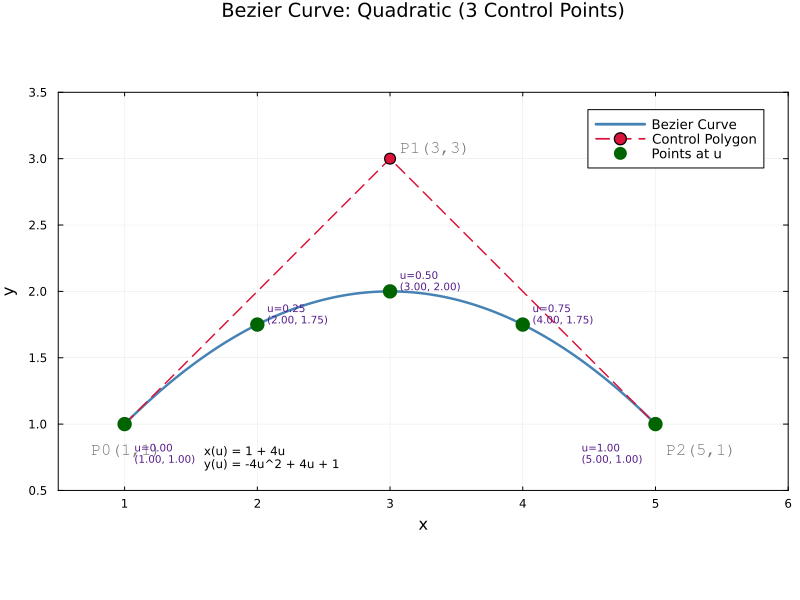
\includegraphics[width=0.95\linewidth]{11-bezier-quadratic-plots.png}
  \caption{Quadratic B\'ezier curve with 3 control points,
           plotted with Plots.jl.}
  \label{fig:bezier-quadratic}
\end{figure}


% =============================================================
\needspace{8\baselineskip}
\section{Reading the Plot}
% =============================================================

\textit{Before looking at a single line of code,
let us understand what is being shown.}

\needspace{5\baselineskip}
\subsection{The three visual elements}

The plot contains three distinct visual layers, each with its
own entry in the legend:

\textbf{Blue solid line --- Bezier Curve.}
This is the actual curve: 200 points computed by evaluating
the parametric equations at $u = 0, \tfrac{1}{199}, \tfrac{2}{199},
\ldots, 1$ and connecting them.
The curve is smooth, starts at $P_0 = (1,1)$, and ends at
$P_2 = (5,1)$.
It does not pass through $P_1 = (3,3)$ --- that point only
pulls the curve upward.

\textbf{Red dashed line with circles --- Control Polygon.}
The straight lines connecting the three control points
$P_0 \to P_1 \to P_2$ form the control polygon.
The red circles mark the exact positions of $P_0$, $P_1$, $P_2$.
The control polygon is the skeleton that shapes the curve.

\textbf{Green dots --- Points at u.}
Five specific points on the curve are highlighted at
$u = 0, 0.25, 0.50, 0.75, 1.00$.
Each green dot sits exactly on the blue curve.

\needspace{5\baselineskip}
\subsection{The annotations}

\textbf{Control point labels (red, bold).}
\cd{P0(1,1)}, \cd{P1(3,3)}, \cd{P2(5,1)} label each
control point.

\textbf{Highlighted point labels (purple).}
Each green dot is annotated with its $u$ value and
coordinates, for example \cd{u=0.50 / (3.00, 2.00)}.
The offsets are carefully chosen to avoid overlapping
the curve or each other.

\textbf{Parametric equations (black, bottom-left).}
The two polynomials are written directly on the plot:
\[
  x(u) = 1 + 4u \qquad y(u) = -4u^2 + 4u + 1
\]
These are the same polynomials derived algebraically in
script~01.

\needspace{5\baselineskip}
\subsection{Geometric observations}

\begin{examplebox}
\textbf{The curve is symmetric.}
The control points $P_0 = (1,1)$ and $P_2 = (5,1)$
are at the same height, and $P_1 = (3,3)$ is exactly
centred between them at $x = 3$.
This produces a perfectly symmetric arc.

\textbf{The midpoint $u = 0.5$ is the peak.}
At $u = 0.5$: $x = 1 + 4(0.5) = 3$, $y = -4(0.25) + 4(0.5) + 1 = 2$.
The green dot at $(3, 2)$ is the highest point on the curve.

\textbf{Points $u = 0.25$ and $u = 0.75$ are mirror images.}
Both sit at $y = 1.75$, symmetric about $x = 3$.
At $u = 0.25$: $x = 2$, $y = 1.75$.
At $u = 0.75$: $x = 4$, $y = 1.75$.

\textbf{The curve always lies within the control polygon.}
This is the convex hull property of B\'ezier curves.
Every point on the curve is a weighted average of the
control points, so it stays inside the triangle
formed by $P_0$, $P_1$, $P_2$.
\end{examplebox}


% =============================================================
\needspace{8\baselineskip}
\section{What is Plots.jl?}
% =============================================================

\textit{Julia has two major plotting libraries.
Understanding which is which helps you read documentation
and choose the right tool.}

\textbf{Plots.jl} is a \emph{plotting metapackage}.
It provides a single, unified API and uses a separate
\emph{backend} to do the actual rendering.
You write \cd{plot(x, y)} and Plots.jl translates that
into calls to GR, PyPlot, Plotly, or other backends.
This means:
\begin{itemize}
  \item One syntax works across multiple backends.
  \item The default backend (GR) requires no extra setup.
  \item It is well-suited for static plots saved to PNG or PDF.
\end{itemize}

\textbf{Makie.jl} (used in scripts~11-makie, 12, 21, 22) is a
\emph{native Julia plotting framework}.
It renders directly without a backend, supports interactive
and GPU-accelerated plots, and has a different API.
CairoMakie renders to files; GLMakie renders in a window.

\begin{notebox}
\textbf{Which should you use?}

Use \textbf{Plots.jl} when you want a simple, familiar
matplotlib-like interface and static output.

Use \textbf{Makie.jl} when you need interactivity,
animations, or high-performance rendering.

This script uses Plots.jl.
Install it once with:
\begin{minted}{julia}
import Pkg; Pkg.add("Plots")
\end{minted}
\end{notebox}


% =============================================================
\needspace{8\baselineskip}
\section{Type Map}
% =============================================================

\tikzset{
  structbox/.style={
    rectangle, rounded corners=4pt,
    draw=MidnightBlue, line width=1.5pt,
    fill=examplebg,
    text width=3.2cm, align=center,
    font=\small\bfseries, inner sep=8pt
  },
  funcbox/.style={
    rectangle, rounded corners=2pt,
    draw=gray!60, line width=1pt,
    fill=white,
    text width=3.2cm, align=center,
    font=\small, inner sep=7pt
  },
  entrybox/.style={
    rectangle, rounded corners=4pt,
    draw=BrickRed, line width=1.5pt,
    fill=notebg,
    text width=2.4cm, align=center,
    font=\small\bfseries, inner sep=8pt
  },
  myarrow/.style={-Stealth, thick, draw=gray!70},
  bluearrow/.style={-Stealth, thick, draw=MidnightBlue},
  redarrow/.style={-Stealth, thick, draw=BrickRed!80},
  arrowlabel/.style={font=\footnotesize\itshape, fill=white, inner sep=2pt}
}

\begin{center}
\begin{tikzpicture}[node distance=1.4cm and 2.6cm]

  \node[structbox] (bz) {%
    \texttt{BezierQuadratic}\\[3pt]
    \footnotesize\normalfont
    \texttt{p0, p1, p2}\\
    \texttt{::Vector\{Float64\}}
  };

  \node[funcbox, below left=1.5cm and 0.4cm of bz] (math) {%
    \textbf{Math functions}\\[2pt]
    \footnotesize\normalfont
    \texttt{basis(u)}\\
    \texttt{point(bz, u)}\\
    \texttt{curve(bz, n)}\\
    \texttt{highlight\_points}
  };

  \node[funcbox, below right=1.5cm and 0.4cm of bz] (draw) {%
    \texttt{draw\_and\_save}\\[2pt]
    \footnotesize\normalfont
    \textit{builds plot layer by layer}\\
    \textit{saves PNG + displays}
  };

  \node[entrybox, right=2.2cm of bz] (main) {%
    \texttt{main()}\\[2pt]
    \footnotesize\normalfont\normalcolor
    \textit{entry point}
  };

  \draw[bluearrow] (bz)   -- node[arrowlabel,above left]{passed to} (math);
  \draw[bluearrow] (bz)   -- node[arrowlabel,above right]{passed to} (draw);
  \draw[myarrow]   (draw) -- node[arrowlabel,below]{calls} (math);
  \draw[redarrow]  (main) -- node[arrowlabel,above]{creates} (bz);
  \draw[redarrow]  (main) |- node[arrowlabel,right,pos=0.8]{calls} (draw);

\end{tikzpicture}
\end{center}

\begin{notebox}
This script has no \cd{BezierExpansion} or polynomial type.
The math is simpler: one struct holds the three control
point vectors, three functions compute curve geometry,
and \cd{draw\_and\_save} handles all plotting.
\end{notebox}


% =============================================================
\needspace{8\baselineskip}
\section{Data and Constants}
% =============================================================

\begin{minted}{julia}
const CONTROL_POINTS = [
    1.0  1.0;   # P0
    3.0  3.0;   # P1
    5.0  1.0;   # P2
]

const U_HIGHLIGHT = [0.00, 0.25, 0.50, 0.75, 1.00]
\end{minted}

\cd{CONTROL\_POINTS} is a $3 \times 2$ matrix.
Each row is one control point; column 1 is $x$,
column 2 is $y$.
The \cd{const} keyword declares a module-level constant ---
its value is fixed for the lifetime of the program.

\cd{U\_HIGHLIGHT} is the list of $u$ values at which the
green dots will be placed.

\begin{minted}{julia}
const COLOR_CURVE   = :steelblue
const COLOR_POLYGON = :crimson
const COLOR_POINT   = :darkgreen
const COLOR_LABEL   = :purple4
const COLOR_CTRL    = :crimson
\end{minted}

Colours in Plots.jl are named with \textbf{Symbol} values
(starting with \cd{:}).
A symbol like \cd{:steelblue} is an interned string ---
Plots.jl recognises CSS colour names and a wide set of
named colours.
Collecting all colour choices in named constants at the
top of the file makes them easy to change without hunting
through the drawing code.


% =============================================================
\needspace{8\baselineskip}
\section{The \texttt{BezierQuadratic} Struct and Constructor}
% =============================================================

\begin{minted}{julia}
struct BezierQuadratic
    p0::Vector{Float64}
    p1::Vector{Float64}
    p2::Vector{Float64}
end

BezierQuadratic(pts::Matrix{Float64}) =
    BezierQuadratic(pts[1,:], pts[2,:], pts[3,:])
\end{minted}

The struct stores the three control points as separate
vectors rather than a matrix.
This makes the math functions easier to read: \cd{bz.p0},
\cd{bz.p1}, \cd{bz.p2} are immediately meaningful.

The outer constructor extracts rows from the matrix using
\textbf{row-slice} syntax: \cd{pts[1,:]} means
``row 1, all columns'' --- a \cd{Vector\{Float64\}} of
length 2 (the $x$ and $y$ coordinates of $P_0$).

\begin{examplebox}
\cd{pts = CONTROL\_POINTS}

\cd{pts[1,:] = [1.0, 1.0]} \quad ($P_0$)

\cd{pts[2,:] = [3.0, 3.0]} \quad ($P_1$)

\cd{pts[3,:] = [5.0, 1.0]} \quad ($P_2$)
\end{examplebox}


% =============================================================
\needspace{8\baselineskip}
\section{The Math Functions}
% =============================================================

\needspace{5\baselineskip}
\subsection{\texttt{basis(u)} --- Bernstein weights}

\begin{minted}{julia}
function basis(u::Float64)
    b0 = (1 - u)^2
    b1 = 2 * u * (1 - u)
    b2 = u^2
    return b0, b1, b2
end
\end{minted}

Returns a \textbf{tuple} of three values --- the three
quadratic Bernstein basis polynomials evaluated at $u$:
\[
  B_0(u) = (1-u)^2, \quad
  B_1(u) = 2u(1-u), \quad
  B_2(u) = u^2
\]

In Julia, \cd{return b0, b1, b2} returns a \cd{Tuple\{Float64, Float64, Float64\}}.
The caller unpacks it with \cd{b0, b1, b2 = basis(u)}.

\begin{examplebox}
\cd{basis(0.5)} $\to$ \cd{(0.25, 0.5, 0.25)}

Check: $0.25 + 0.5 + 0.25 = 1.0$ \checkmark
(partition of unity)
\end{examplebox}

\needspace{5\baselineskip}
\subsection{\texttt{point(bz, u)} --- one point on the curve}

\begin{minted}{julia}
function point(bz::BezierQuadratic, u::Float64)
    b0, b1, b2 = basis(u)
    b0 .* bz.p0 .+ b1 .* bz.p1 .+ b2 .* bz.p2
end
\end{minted}

Evaluates the curve at parameter $u$:
\[
  P(u) = B_0(u) \cdot P_0 + B_1(u) \cdot P_1 + B_2(u) \cdot P_2
\]

The dot operators \cd{.*} and \cd{.+} are
\textbf{broadcast} operations --- they apply element-wise
to vectors.
\cd{b0 .* bz.p0} multiplies the scalar \cd{b0} by each
element of the vector \cd{bz.p0},
giving a scaled 2-D vector.
The three scaled vectors are then added element-wise.

The result is a \cd{Vector\{Float64\}} of length 2:
the $[x, y]$ coordinates of the curve at $u$.

\begin{examplebox}
At $u = 0.5$:

\cd{b0, b1, b2 = 0.25, 0.5, 0.25}

\cd{0.25 .* [1,1] .+ 0.5 .* [3,3] .+ 0.25 .* [5,1]}

$= [0.25, 0.25] + [1.5, 1.5] + [1.25, 0.25]$

$= [3.0, 2.0]$ \checkmark
\end{examplebox}

\needspace{5\baselineskip}
\subsection{\texttt{curve(bz, n)} --- the full curve as a matrix}

\begin{minted}{julia}
function curve(bz::BezierQuadratic, n::Int=200)
    u_vals = LinRange(0.0, 1.0, n)
    pts    = hcat([point(bz, u) for u in u_vals]...)'
    return pts
end
\end{minted}

\textbf{\cd{LinRange(0.0, 1.0, n)}:}
Creates $n$ evenly-spaced values from 0 to 1 inclusive.
With $n = 200$: $[0, \tfrac{1}{199}, \tfrac{2}{199}, \ldots, 1]$.
\cd{LinRange} is memory-efficient --- it does not allocate
a full array but computes each value on demand.

\textbf{The list comprehension:}
\cd{[point(bz, u) for u in u\_vals]} produces a vector
of 200 two-element vectors --- one per $u$ value.

\textbf{\cd{hcat(......)'}:}
This is the most compact part.
\cd{hcat(v1, v2, ...)} \textbf{horizontally concatenates}
vectors into a matrix.
The \cd{...} (splat operator) unpacks the list of 200
vectors into 200 separate arguments to \cd{hcat}.
The result is a $2 \times 200$ matrix.
Transposing with \cd{'} gives a $200 \times 2$ matrix ---
200 rows, each a point $(x, y)$.

\begin{examplebox}
With $n = 3$ for simplicity:

\cd{u\_vals = [0.0, 0.5, 1.0]}

Comprehension gives: \cd{[[1.0,1.0], [3.0,2.0], [5.0,1.0]]}

\cd{hcat([1.0,1.0], [3.0,2.0], [5.0,1.0])} =
$\begin{bmatrix} 1 & 3 & 5 \\ 1 & 2 & 1 \end{bmatrix}$ (shape $2 \times 3$)

After \cd{'} (transpose): shape $3 \times 2$ ---
three rows, each a $(x, y)$ point.
\end{examplebox}

\needspace{5\baselineskip}
\subsection{\texttt{highlight\_points(bz, u\_list)}}

\begin{minted}{julia}
function highlight_points(bz::BezierQuadratic,
                          u_list::Vector{Float64})
    hcat([point(bz, u) for u in u_list]...)'
end
\end{minted}

Identical in structure to \cd{curve}, but takes an
explicit list of $u$ values instead of generating them.
Returns an $m \times 2$ matrix of the $m$ highlighted
points.
Used to place the green dots at $u = 0, 0.25, 0.5, 0.75, 1$.


% =============================================================
\needspace{8\baselineskip}
\section{Annotation Offsets}
% =============================================================

\begin{minted}{julia}
const U_OFFSETS = Dict(
    0.00 => ( 0.08, -0.22),
    0.25 => ( 0.08,  0.08),
    0.50 => ( 0.08,  0.08),
    0.75 => ( 0.08,  0.08),
    1.00 => (-0.55, -0.22),
)
\end{minted}

Each annotation label is placed at an offset
$(dx, dy)$ from the point it annotates.
The offsets are hand-tuned to prevent labels from
overlapping the curve or each other.

The $u = 0$ label shifts down (\cd{dy = -0.22}) because
the curve starts at the bottom-left and there is room below.
The $u = 1$ label shifts left (\cd{dx = -0.55}) to
avoid going off the right edge of the plot.
All intermediate labels shift up-right (\cd{0.08, 0.08}).


% =============================================================
\needspace{8\baselineskip}
\section{\texttt{draw\_and\_save} --- Building the Plot}
% =============================================================

\textit{This is the main plotting function.
It builds the figure layer by layer, with each
\cd{plot!} or \cd{scatter!} call adding one visual element.
The exclamation mark \cd{!} is a Julia convention meaning
``modify in place'' --- it adds to the existing plot
rather than creating a new one.}

\needspace{5\baselineskip}
\subsection{Creating the base figure}

\begin{minted}{julia}
plt = plot(
    size         = (800, 600),
    background   = :white,
    grid         = true,
    gridalpha    = 0.3,
    gridcolor    = :lightgray,
    framestyle   = :box,
    xlims        = (0.5, 6.0),
    ylims        = (0.5, 3.5),
    aspect_ratio = :equal,
    xlabel       = "x",
    ylabel       = "y",
    title        = "Bezier Curve: Quadratic (3 Control Points)",
    titlefontsize = 13,
    labelfontsize = 11,
    legend       = :topright,
    legendfontsize = 9,
)
\end{minted}

\cd{plot()} with no data creates an empty figure with
all the layout settings applied.
Key attributes:

\begin{itemize}
  \item \cd{size = (800, 600)} --- pixel dimensions of the saved PNG.
  \item \cd{framestyle = :box} --- draws a box around all four sides,
        giving the plot the framed appearance visible in the output.
  \item \cd{aspect\_ratio = :equal} --- forces the $x$ and $y$ axes
        to use the same scale per unit, so the curve is not distorted.
        Without this, a circle would look like an ellipse.
  \item \cd{xlims}, \cd{ylims} --- set the visible range.
        The data goes from $x=1$ to $x=5$ and $y=1$ to $y=3$;
        these limits add padding around it.
  \item \cd{legend = :topright} --- places the legend in the
        top-right corner, where there is space between the
        curve and the control polygon.
\end{itemize}

\needspace{5\baselineskip}
\subsection{Adding the curve}

\begin{minted}{julia}
cpts = curve(bz)
plot!(plt,
    cpts[:,1], cpts[:,2],
    color     = COLOR_CURVE,
    linewidth = 2.5,
    label     = "Bezier Curve",
)
\end{minted}

\cd{cpts[:,1]} is the column-slice for all $x$ coordinates
(column 1 of the $200 \times 2$ matrix).
\cd{cpts[:,2]} is all $y$ coordinates.
Passing two vectors to \cd{plot!} draws a line through
those points.

\cd{label = "Bezier Curve"} is what appears in the legend.
If you pass \cd{label = ""} or \cd{label = false},
the element is excluded from the legend.

\begin{examplebox}
\textbf{Actual content of \cd{cpts} (first 5 and last 2 rows shown):}

\cd{cpts} is a $200 \times 2$ matrix.
Each row is one $(x, y)$ point on the curve.

\medskip
\begin{center}
\begin{tabular}{rcc}
\toprule
Row & \cd{cpts[:,1]} ($x$) & \cd{cpts[:,2]} ($y$) \\
\midrule
1   & 1.0000 & 1.0000 \\
2   & 1.0402 & 1.0793 \\
3   & 1.0804 & 1.1571 \\
4   & 1.1206 & 1.2334 \\
5   & 1.1608 & 1.3082 \\
$\vdots$ & $\vdots$ & $\vdots$ \\
100 & 3.0000 & 2.0000 \\
$\vdots$ & $\vdots$ & $\vdots$ \\
199 & 4.9598 & 1.0793 \\
200 & 5.0000 & 1.0000 \\
\bottomrule
\end{tabular}
\end{center}

\medskip
\cd{cpts[:,1] = [1.0, 1.040, 1.080, ..., 3.0, ..., 5.0]}
\quad --- the $x$ vector passed to \cd{plot!}

\cd{cpts[:,2] = [1.0, 1.079, 1.157, ..., 2.0, ..., 1.0]}
\quad --- the $y$ vector passed to \cd{plot!}
\end{examplebox}

\needspace{5\baselineskip}
\subsection{Adding the control polygon}

\begin{minted}{julia}
cp = vcat(bz.p0', bz.p1', bz.p2')
plot!(plt,
    cp[:,1], cp[:,2],
    color      = COLOR_POLYGON,
    linestyle  = :dash,
    linewidth  = 1.5,
    marker     = :circle,
    markersize = 6,
    label      = "Control Polygon",
)
\end{minted}

\cd{bz.p0'} transposes the length-2 vector \cd{[1.0, 1.0]}
into a $1 \times 2$ row vector.
\cd{vcat(bz.p0', bz.p1', bz.p2')} stacks three row
vectors into a $3 \times 2$ matrix --- exactly the shape
needed to plot the polygon.

\cd{marker = :circle} draws a circle at each data point
(the control points).
\cd{linestyle = :dash} produces the dashed red line
connecting them.
By setting both \cd{color} and \cd{marker} on the same
\cd{plot!} call, the line and the markers share the same
colour --- which is why the control polygon line and dots
are both crimson.

\begin{examplebox}
\textbf{Actual content of \cd{cp}:}

\[
  \cd{cp} =
  \begin{bmatrix}
    1.0 & 1.0 \\
    3.0 & 3.0 \\
    5.0 & 1.0
  \end{bmatrix}
  \quad \text{shape } 3 \times 2
\]

\cd{cp[:,1] = [1.0, 3.0, 5.0]} \quad --- $x$ coordinates of $P_0$, $P_1$, $P_2$

\cd{cp[:,2] = [1.0, 3.0, 1.0]} \quad --- $y$ coordinates of $P_0$, $P_1$, $P_2$

These two vectors define the three corners of the dashed
red control polygon.
Plots.jl connects them in order: $(1,1) \to (3,3) \to (5,1)$.
\end{examplebox}

\needspace{5\baselineskip}
\subsection{Annotating control points}

\begin{minted}{julia}
offsets_ctrl = [(-0.25, -0.20), (0.08, 0.08), (0.08, -0.20)]
names_ctrl   = ["P0(1,1)", "P1(3,3)", "P2(5,1)"]
for (pt, name, (dx, dy)) in zip(eachrow(cp), names_ctrl, offsets_ctrl)
    annotate!(plt,
        pt[1] + dx, pt[2] + dy,
        text(name, COLOR_CTRL, :left, 9, :bold)
    )
end
\end{minted}

\textbf{\cd{eachrow(cp)}:}
Returns an iterator over the rows of the matrix \cd{cp}.
Each iteration gives one row as a vector --- one control point.

\textbf{\cd{zip(eachrow(cp), names\_ctrl, offsets\_ctrl)}:}
Zips three iterables together.
Each iteration yields a tuple of one row, one name string,
and one offset pair.
The pattern \cd{(dx, dy)} in the loop variable
\textbf{destructures} the offset tuple directly.

\textbf{\cd{annotate!(plt, x, y, text(...))}:}
Places a text label at position \cd{(x, y)}.
The \cd{text()} function specifies the string, colour,
alignment (\cd{:left}), font size (9), and style (\cd{:bold}).

\needspace{5\baselineskip}
\subsection{Adding the highlighted points}

\begin{minted}{julia}
hpts = highlight_points(bz, u_highlight)
scatter!(plt,
    hpts[:,1], hpts[:,2],
    color             = COLOR_POINT,
    markersize        = 8,
    markerstrokewidth = 0,
    label             = "Points at u",
)
\end{minted}

\cd{scatter!} adds a scatter plot (markers only, no line).
\cd{markerstrokewidth = 0} removes the border around each
marker, giving the filled green circles visible in the plot.

\begin{examplebox}
\textbf{Actual content of \cd{hpts}:}

\[
  \cd{hpts} =
  \begin{bmatrix}
    1.00 & 1.00 \\
    2.00 & 1.75 \\
    3.00 & 2.00 \\
    4.00 & 1.75 \\
    5.00 & 1.00
  \end{bmatrix}
  \quad \text{shape } 5 \times 2
\]

Each row is one green dot.
Reading down: $u=0, 0.25, 0.50, 0.75, 1.00$.

\cd{hpts[:,1] = [1.0, 2.0, 3.0, 4.0, 5.0]} \quad --- $x$ coords of the five dots

\cd{hpts[:,2] = [1.0, 1.75, 2.0, 1.75, 1.0]} \quad --- $y$ coords of the five dots

The $y$ values confirm the symmetry: $u=0.25$ and $u=0.75$
both give $y=1.75$, and $u=0.50$ gives the peak at $y=2.00$.
\end{examplebox}

\needspace{5\baselineskip}
\subsection{Annotating highlighted points}

\begin{minted}{julia}
for u in u_highlight
    pt     = point(bz, u)
    x, y   = pt[1], pt[2]
    dx, dy = get(U_OFFSETS, u, (0.08, 0.08))
    lbl    = @sprintf("u=%.2f\n(%.2f, %.2f)", u, x, y)
    annotate!(plt,
        x + dx, y + dy,
        text(lbl, COLOR_LABEL, :left, 7)
    )
end
\end{minted}

For each $u$ value, this computes the point, looks up the
offset from \cd{U\_OFFSETS} (falling back to \cd{(0.08, 0.08)}
if not found), formats the label string with two lines
using \cd{\\n} for a line break, and places the annotation.

\cd{@sprintf("u=\%.2f\\n(\%.2f, \%.2f)", u, x, y)} formats
the $u$ value and coordinates each to 2 decimal places,
producing strings like \cd{"u=0.50\\n(3.00, 2.00)"}.

\begin{examplebox}
\textbf{Value of \cd{pt = point(bz, u)} for each iteration:}

\medskip
\begin{tabular}{cccll}
\toprule
$u$ & \cd{pt[1]} ($x$) & \cd{pt[2]} ($y$) & \cd{lbl} string & offset $(dx,dy)$ \\
\midrule
0.00 & 1.00 & 1.00 & \cd{"u=0.00\textbackslash n(1.00, 1.00)"} & $(+0.08, -0.22)$ \\
0.25 & 2.00 & 1.75 & \cd{"u=0.25\textbackslash n(2.00, 1.75)"} & $(+0.08, +0.08)$ \\
0.50 & 3.00 & 2.00 & \cd{"u=0.50\textbackslash n(3.00, 2.00)"} & $(+0.08, +0.08)$ \\
0.75 & 4.00 & 1.75 & \cd{"u=0.75\textbackslash n(4.00, 1.75)"} & $(+0.08, +0.08)$ \\
1.00 & 5.00 & 1.00 & \cd{"u=1.00\textbackslash n(5.00, 1.00)"} & $(-0.55, -0.22)$ \\
\bottomrule
\end{tabular}

\medskip
Each annotation is placed at \cd{(pt[1]+dx, pt[2]+dy)}.
For $u=0.50$: annotation at $(3.00+0.08,\; 2.00+0.08) = (3.08, 2.08)$,
just above and to the right of the green dot.
\end{examplebox}

\needspace{5\baselineskip}
\subsection{Adding the equation text}

\begin{minted}{julia}
annotate!(plt,
    1.6, 0.75,
    text("x(u) = 1 + 4u\ny(u) = -4u^2 + 4u + 1",
         :black, :left, 8)
)
\end{minted}

A free-floating text annotation at position $(1.6, 0.75)$,
just below the main plot area.
The coordinates are in data units (the same coordinate
system as the axes), not pixels.

\needspace{5\baselineskip}
\subsection{Saving and displaying}

\begin{minted}{julia}
savefig(plt, filename)
println("Saved: $filename")
display(plt)
println("Press Enter to close...")
readline()
\end{minted}

\cd{savefig(plt, filename)} saves the plot to a PNG file.
The filename extension \cd{.png} tells Plots.jl to use
the PNG format.

\cd{display(plt)} opens the plot in a window (using the
active backend's display system).

\cd{readline()} pauses execution and waits for the user
to press Enter.
Without this, the script would exit immediately and the
window would close before you could see the plot.


% =============================================================
\needspace{8\baselineskip}
\section{Entry Point}
% =============================================================

\begin{minted}{julia}
function main()
    bz = BezierQuadratic(CONTROL_POINTS)
    draw_and_save(bz, U_HIGHLIGHT, "11-bezier-quadratic-plots.png")
end

main()
\end{minted}

\cd{BezierQuadratic(CONTROL\_POINTS)} calls the outer
constructor, extracting the three row vectors from the matrix.

\cd{draw\_and\_save} does everything else: computes the
curve, adds all plot layers, saves the PNG, and waits
for the user.

\begin{notebox}
\textbf{How to run:}
\begin{minted}{julia}
julia 11-bezier-quadratic-plots.jl
\end{minted}
The script displays the plot in a window and saves
\cd{11-bezier-quadratic-plots.png} in the current directory.
Press Enter in the terminal to close the window and exit.
\end{notebox}

\vspace{2em}\hrule\vspace{0.5em}
{\small\textcolor{gray}{%
Explanation for \texttt{11-bezier-quadratic-plots.jl}
\textbar{} Directed and curated by E.R.\ Nurwijayadi
\textbar{} Code and explanations AI-generated}}

\end{document}
